\documentclass[reprint,english,notitlepage]{revtex4-2}
\usepackage{amsmath}
\usepackage[mathletters]{ucs}
\usepackage[utf8x]{inputenc}
\usepackage[english]{babel}
\usepackage{esint}
\usepackage{physics,amssymb}
\usepackage{graphicx}
\usepackage{xcolor}
\usepackage{hyperref}
\usepackage{listings}
\usepackage{subfigure}
% \usepackage[style=science, backend=biber]{biblatex}
% \addbibresource{References_Part_4.bib} TODO: Slett før innlevering
\hypersetup{
    colorlinks,
    linkcolor={red!50!black},
    citecolor={blue!50!black},
    urlcolor={blue!80!black}}

\lstset{inputpath=,
    backgroundcolor=\color{white!88!black},
    basicstyle={\ttfamily\scriptsize},
    commentstyle=\color{magenta},
    language=Python,
    morekeywords={True,False},
    tabsize=4,
    stringstyle=\color{green!55!black},
    frame=single,
    keywordstyle=\color{blue},
    showstringspaces=false,
    columns=fullflexible,
    keepspaces=true}

\begin{document}

\title{Satellite Launch}
\author{Oskar Idland \& Jannik Eschler}
\date{\today}
\affiliation{Institute of Theoretical Astrophysics, University of Oslo}

\begin{abstract}
    This is an abstract \colorbox{red}{Complete this summary at the end of the paper} 
\end{abstract}
\maketitle

\section{Introduction} \label{sec:introduction}
The purpose of this project is the launch of our shuttle.
Interplanetary travel have huge cost and risks.
Therefore we must guarantee success by planning ahead of our journey.
We will develop a simulation to visualize our orbit given some parameters as a means to get a good picture of where we will end up.

\section{Theory} \label{sec: theory}
\colorbox{red}{Refferer til forklaring av leapfrog fra tidligere deler}

\section{Method} \label{sec: method}
\subsection{Simulating trajectory} \label{ssec: simulating trajectory}
To simulate the trajectory our 

% Metode som kan brukes om ting blir simulert som N-body system. Hvis ikke bruk det som står over
% shuttle will have we simplify our system into a N-body system where all the planets and star will be combined into a single body. As the mass of the shuttle is so small in comparison to the rest of our solar system, we will disregard its gravitational pull. First we will calculate the center of mass $ \mathbf{CM} $
% \[
% \mathbf{CM} = \frac{1}{M} \sum_{i} m_i \mathbf{r_i}
% \]
% where $ M $ is the total mass of our solar system and $ m_i $ and $ r_i $ is the mass and position of each planet respectively. We then find the total momentum $ \mathbf{p} $ as a sum of all the momentum of each planet in the system
% \[
% \mathbf{p} = \sum_{i} m_i \mathbf{v_i}
% \]
% where $ \mathbf{v_i} $ is the velocity of each planet. 
% As we use the position of the star as origin we represent the position of the $ \mathbf{CM} $ as $ \mathbf{r}_{sys} $. This position changes over time with a velocity $ \mathbf{v}_{sys} = \frac{\mathbf{p}}{M} $.  
% As the shuttle travels, its position $ \mathbf{r} $ will be influenced by its initial velocity $ \mathbf{v_0} $ and the gravitational pull of the system. The acceleration of the spacecraft is given by 
% \[
% \mathbf{a} = -G \frac{M}{\left\vert \mathbf{r} - \mathbf{r}_{sys} \right\vert ^{3}} (\mathbf{r} - \mathbf{r}_{sys}).
% \]
Using the leapfrog method for numerical integration we can calculate the full trajectory of our shuttle.
\newline
\subsection{Getting close enough to the target planet}
To make our journey as easy as possible we first try to check where our home planet and target planet are the closest. Using the orbits calculated from \colorbox{red}{Refferer til Part 2 kalkulasjoner} we iterate over all positions and check at which time $ t_{0} $ the distance is the smallest. With this position it seems favorable to launch from the bottom of our planet $ \mathbf{r}_0 $. To figure out the direction to launch our planet we begin by using an educated guess by pointing the shuttle directly at the target planet. We then continue by simulating the orbit for multiple, evenly spaced out angles from the angle of the vector pointing directly at the target planet $ \mathbf{v}_0 $, to a max angle of $ π/8 $ radians just to get a picture of how the launch will look for different angles.  Now we have a wide span of possible angles. Before narrowing the angles down we will iterater over possible values for $ \left\vert \mathbf{v}_0 \right\vert  $. This gives us an idea of how fast the shuttle needs to travel for it to get even close to reaching the target planet. Once this is done, we will iterate over a range of angles and velocities, find the time we are the closest to the target planet and the distance. For each case we will check if the smallest distance $ d $ satisfy the requirement for beginning orbit around target planet given by 
\[
d \le l, \qquad l = \left\vert \mathbf{r} \right\vert \sqrt{\frac{M_{target}}{M_{star}}}  
\]


\section{Results} \label{sec: results}
\begin{figure}[h!]
  \centering
  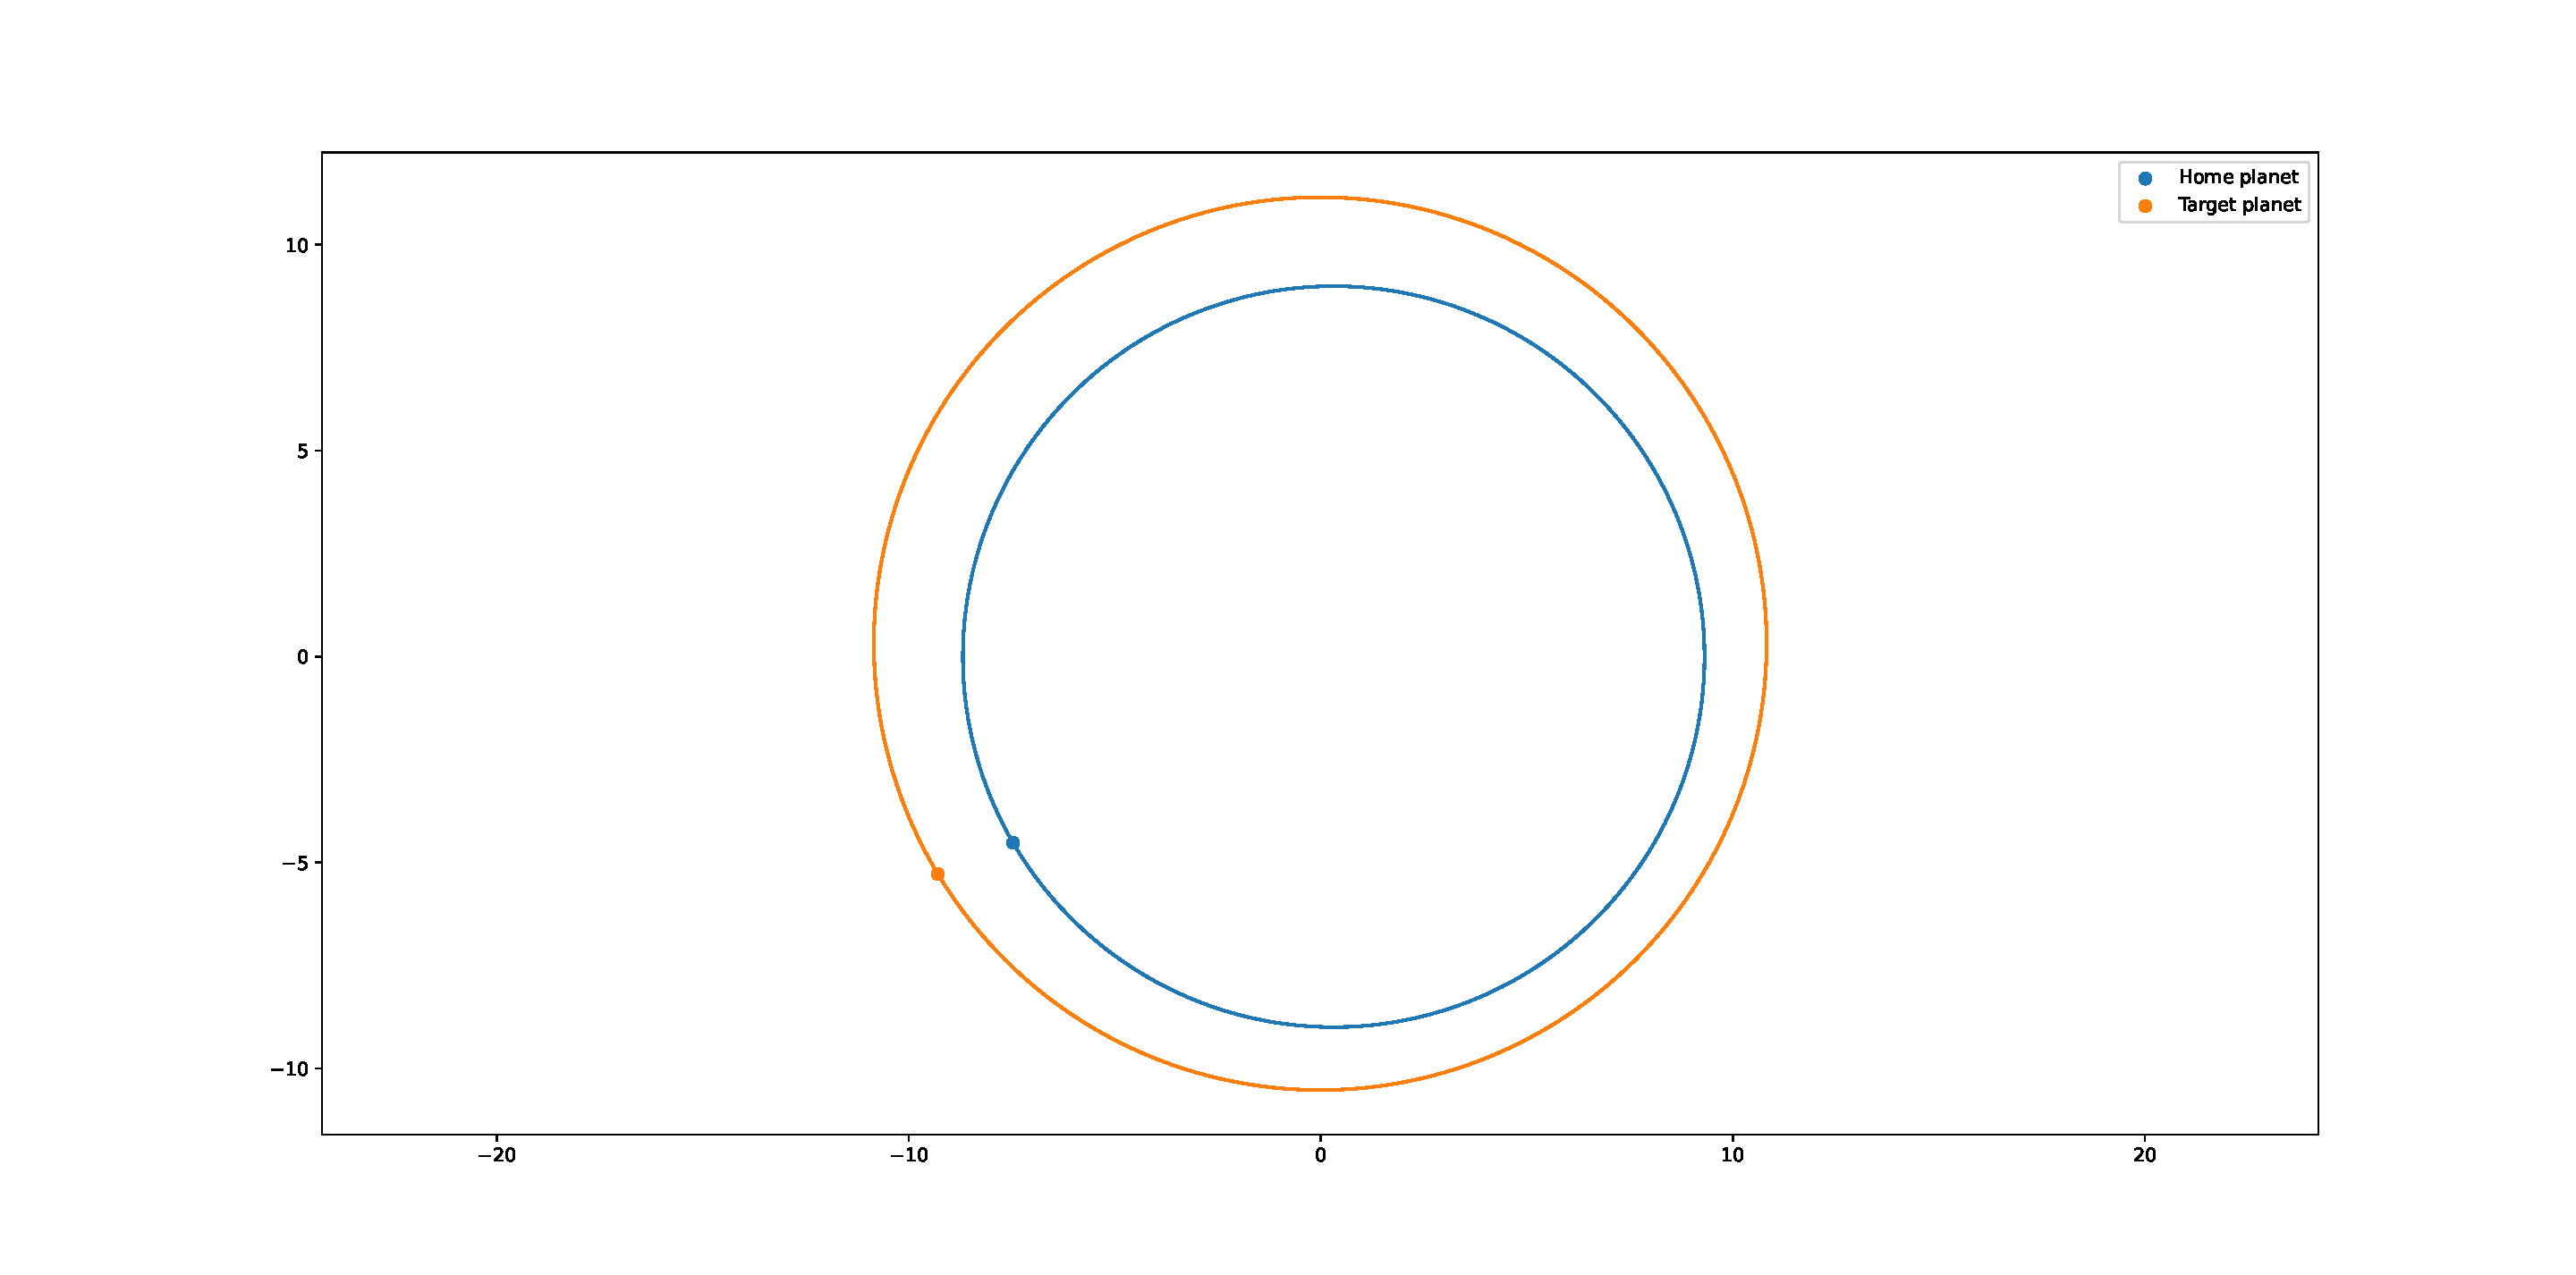
\includegraphics[scale = .18]{Figures/closest_orbit.pdf}
  \caption{Position where the target planet and our home planet were the closest}
  \label{fig: closest orbit}
\end{figure}
\section{Discussion} \label{sec: discussion}

\section{Conclusion} \label{sec: conclusion}

\section{Appendix} \label{sec: appendix}

\section*{ACKNOWLEDGMENTS}

\section*{References} \label{sec: references}
% printbibliography TODO: Remove Comment
\end{document}